\chapter{植物生活：扎根生长，欣欣向荣}\label{ch:g12:plant-rooted-life}

橡树不能走到水边，也不能躲开毛毛虫，
也不能外出寻找配偶。它在橡子落下的地方扎根三个世纪，
这期间汲取数百吨水，
抵御成千上万种想要啃食它的\omterm{def:g10:biodiversity-scales:species}{物种}，让叶片朝向光，
并借助风和松鸦，把花粉与橡子散布到四方。
扎根的生活并不被动，它是应对同样问题的另一套方案——
取食、防御、移动、繁殖——
本章即逐一考察。

\section{身体为交换而构造}

\begin{proposition}[两套系统，两种表面]\label{prop:g12:plant-rooted-life:surfaces}
开花植物由两套系统组成：位于土壤中的\emph{根系}，
吸收水分和无机离子并固定植株；
位于空气中的\emph{茎叶系统}——即茎和叶——
它负责吸收光和二氧化碳。二者都是巨大的交换
表面：一棵大树的叶片向光铺开数百平方米的
受光面，其根系则借数十亿条
微小的\emph{根毛}\index{根毛}延伸，
使其与土壤接触的面积也达数百平方米。植物首先是一种
从固定点出发、向两个方向铺展表面的方式。
\end{proposition}
\begin{proof}[证据]
在一箱土壤中培育四个月的单株黑麦，
经测定有 $\num{1.4e10}$ 条\omterm{prop:g12:plant-rooted-life:surfaces}{根毛}，总长超过
\qty{10000}{km}，表面积约 \qty{400}{m^2}，
是其叶面积的十倍。成年橡树约有 250\,000 片叶；一公顷森林
向天空呈现的叶面积为 \qtyrange{5}{8}{ha}。
切除幼苗\omterm{prop:g12:plant-rooted-life:surfaces}{根毛}或包覆叶片，
数日之内便会使其生长停止。
\end{proof}

\begin{omfigure}
\begin{tikzpicture}
  \node[anchor=south west, inner sep=0] (img) at (0,0)
    {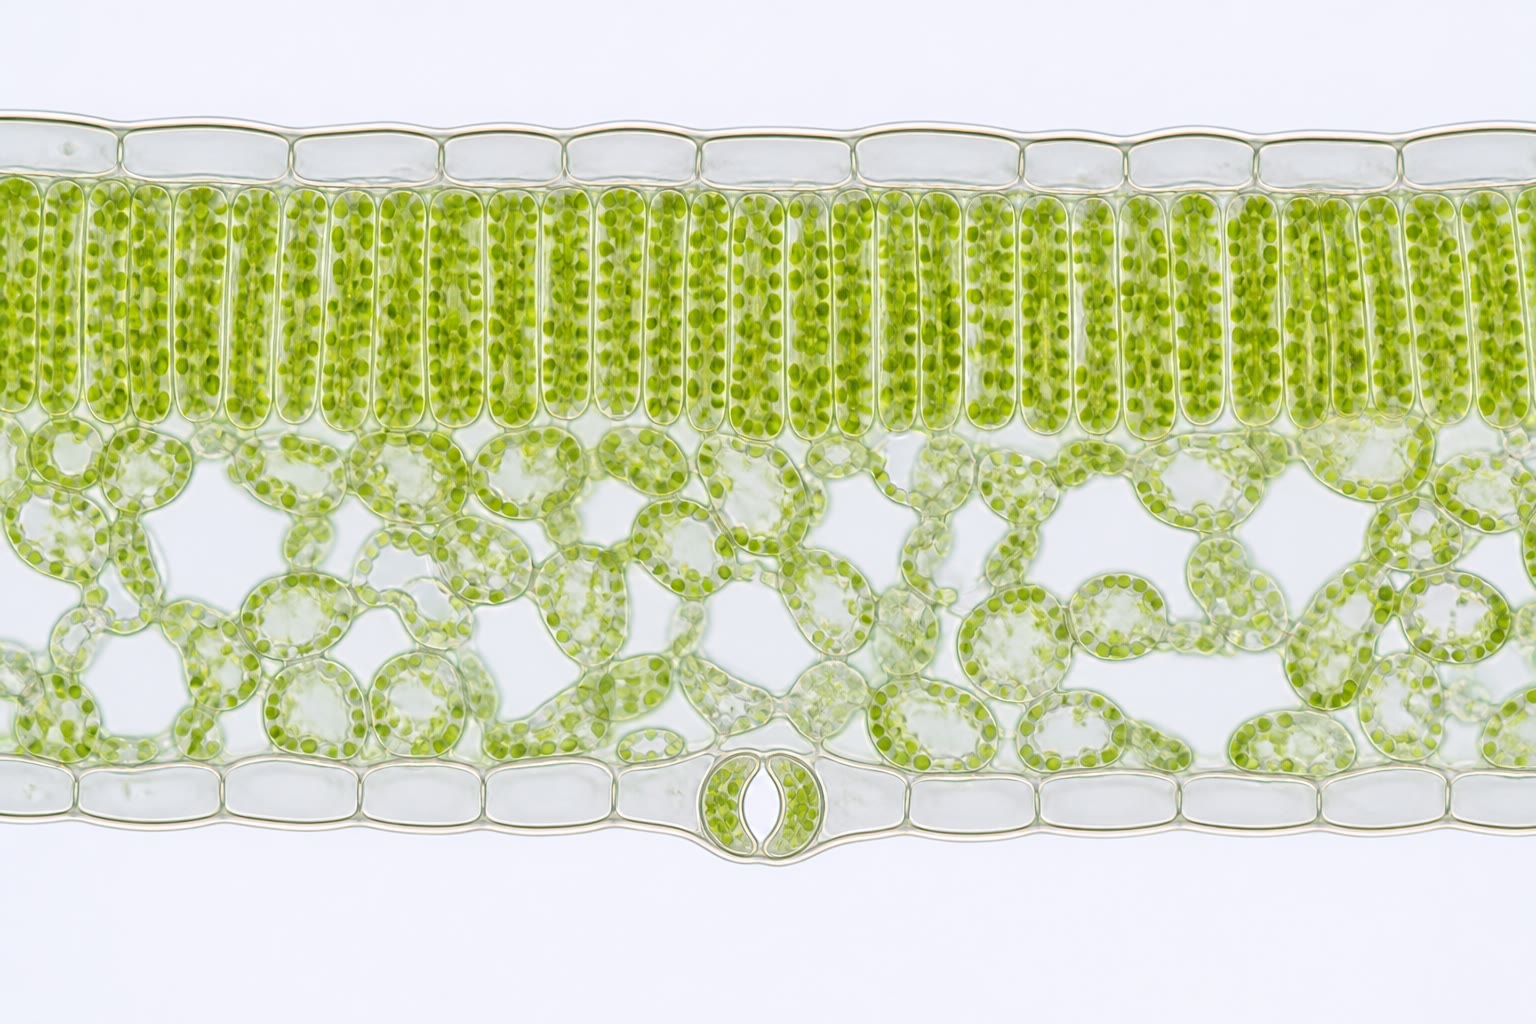
\includegraphics[width=0.56\linewidth]{images/book2/ai/fig-leaf-cross-section.jpg}};
  \begin{scope}[x={(img.south east)}, y={(img.north west)},
      every node/.style={font=\small}]
    \draw[omDef, thick] (0.50,0.88) -- (0.50,1.08) node[above] {角质层和上表皮};
    \draw[omDef, thick] (0.20,0.72) -- (-0.04,0.85) node[left, align=right] {栅栏细胞，\\ 富含叶绿体};
    \draw[omDef, thick] (0.20,0.42) -- (-0.04,0.30) node[left, align=right] {海绵层 \\ 含气隙};
    \draw[omDef, thick] (0.50,0.20) -- (0.50,-0.06) node[below] {两个保卫细胞之间的气孔（下表皮）};
    \draw[omDef, thick] (0.85,0.12) -- (1.04,0.05) node[right] {下表皮};
  \end{scope}
\end{tikzpicture}

{\small 叶的横切面。光线透过透明的上表皮
进入排满\omterm{def:g10:cells-common-unit:organelle}{叶绿体}的栅栏\omterm{def:g10:cells-common-unit:cell}{细胞}；二氧化碳
经下表皮的\omterm{def:g12:plant-rooted-life:stomata}{气孔}进入，并穿过海绵层的气隙扩散
至需要它的\omterm{def:g10:cells-common-unit:cell}{细胞}。}
\end{omfigure}

\begin{definition}[气孔]\label{def:g12:plant-rooted-life:stomata}
称\emph{气孔}\index{气孔}为叶片表皮上的一个小孔，
其两侧由两个\emph{保卫\omterm{def:g10:cells-common-unit:cell}{细胞}}围成，靠膨胀而开、
靠收缩而闭。张开的气孔使二氧化碳得以进入，供\omterm{def:g10:cell-metabolism:autotrophy}{光合作用}；
水汽也随之外逸——即植物取食时无法避免的
\emph{蒸腾作用}。每平方毫米叶片上约有一百至三百个气孔，
多位于下表皮；
它们在光照下张开，在黑暗与干旱时关闭。
\end{definition}

\begin{omfigure}
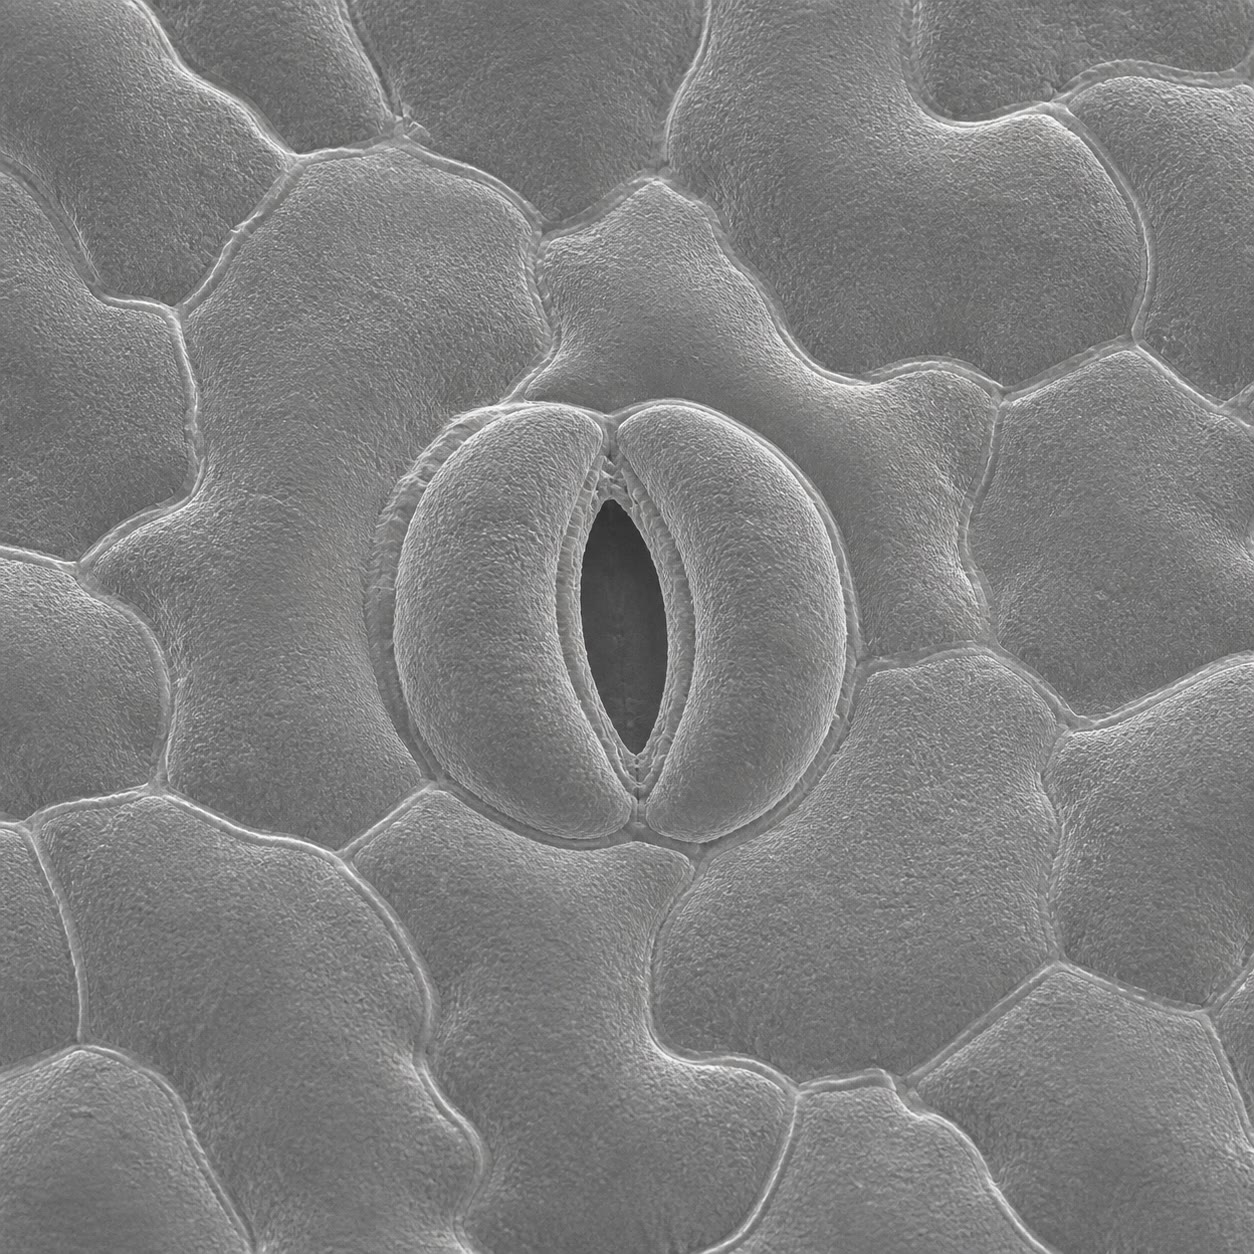
\includegraphics[width=0.4\linewidth]{images/book2/ai/g12-plant-stoma-sem.jpg}

{\small 扫描电子显微镜下的一个\omterm{def:g12:plant-rooted-life:stomata}{气孔}：
孔周围是两个肾形保卫\omterm{def:g10:cells-common-unit:cell}{细胞}，置于叶表皮的扁平\omterm{def:g10:cells-common-unit:cell}{细胞}之间。
孔径只有几微米。}
\end{omfigure}

\begin{omfigure}
\begin{tikzpicture}
\begin{axis}[
  width=0.86\linewidth, height=5.4cm,
  axis x line=bottom, axis y line=left,
  xmin=0, xmax=24, ymin=0, ymax=110,
  xlabel={一天中的小时}, ylabel={占最大值的\%},
  xlabel style={font=\small, at={(axis description cs:0.5,-0.12)}, anchor=north},
  ylabel style={font=\small},
  tick label style={font=\small}, xtick={0,6,12,18,24}, ytick={0,50,100},
  legend style={at={(0.5,-0.3)}, anchor=north, legend columns=3, font=\small, draw=none},
]
\addplot[thick, omProp, smooth] coordinates {(0,0) (5,0) (6,20) (8,80) (12,100) (16,80) (19,20) (20,0) (24,0)};
\addplot[thick, omMeth, smooth] coordinates {(0,5) (5,5) (7,60) (9,95) (13,90) (15,40) (17,70) (19,30) (20,5) (24,5)};
\addplot[thick, omDef, dashed, smooth] coordinates {(0,3) (5,3) (7,50) (9,85) (13,100) (15,45) (17,65) (19,25) (20,3) (24,3)};
\legend{光, 气孔开放, 蒸腾作用}
\end{axis}
\end{tikzpicture}

{\small 叶片的一个夏日。\omterm{def:g12:plant-rooted-life:stomata}{气孔}随光线张开，
夜间关闭；炎热的午后，它们部分关闭以减少失水，
蒸腾作用——随\omterm{def:g12:plant-rooted-life:stomata}{气孔}开放而变化——也随之
下降。}
\end{omfigure}

\section{无心脏的水分与养分运输}

\begin{proposition}[两种汁液]\label{prop:g12:plant-rooted-life:saps}
植物有两套运输系统，皆由长形\omterm{def:g10:cells-common-unit:cell}{细胞}
连接成管，分布于每个器官的维管束中。
\begin{itemize}
  \item \emph{木质部}\index{木质部}输送\emph{原汁液}——水分与
        根所吸收的无机离子——向上运至
        叶片。动力来自蒸腾作用：水分从叶片\omterm{def:g10:cells-common-unit:cell}{细胞}蒸发，
        拉动\omterm{prop:g12:plant-rooted-life:saps}{木质部}中连续的水柱由根部向上，
        如灯芯吸油。无需泵，
        也无需植物耗费能量：提升水柱的是太阳。
  \item \emph{韧皮部}\index{韧皮部}输送\emph{加工汁液}——
        含叶片所制糖分的水——从叶片
        运往一切消耗或储存它们的器官：生长的
        顶端、根、果实、种子与块茎。它由源流向库，
        方向取决于库所在的位置。
\end{itemize}
\end{proposition}
\begin{proof}[证据]
将切下的茎插入染色水中，可见染料沿\omterm{prop:g12:plant-rooted-life:saps}{木质部}上升，
在蒸腾的枝条中比套在袋中的枝条更快；去掉叶片的枝条
则提不起任何水分。剥去一圈树皮（内含\omterm{prop:g12:plant-rooted-life:saps}{韧皮部}）
自树干剥下后，使糖分不能抵达根部，根
数月内便会饿死，而环剥以上的叶片仍能获得水分；
糖分在环剥以上积累，树皮随之膨大。蚜虫
以针状口器取食\omterm{prop:g12:plant-rooted-life:saps}{韧皮部}，若将口针切断，
便会从口针中流出一滴带压的含糖汁液。
\end{proof}

\begin{omfigure}
\begin{tikzpicture}[font=\small, >=Stealth, line cap=round]
  % plant: roots, stem, leaves, fruit
  \draw[line width=6pt, omProp!40] (0,0) -- (0,5.5);           % stem
  \draw[thick, fill=omMeth!40] (0,4.6) .. controls (-1.2,5.0) and (-1.6,4.0) .. (-0.2,3.9) -- cycle;   % left leaf
  \draw[thick, fill=omMeth!40] (0,3.4) .. controls (1.2,3.8) and (1.6,2.8) .. (0.2,2.7) -- cycle;      % right leaf
  \draw[thick, fill=omThm!40] (0.9,5.4) circle (0.35);                                                 % fruit
  \draw[thick, omProp!60] (0,5.5) -- (0.7,5.3);
  \foreach \a in {-150,-120,-90,-60,-30} \draw[thick, omProp!70] (0,0) -- (\a:1.8);                   % roots
  \node[anchor=north] at (0,-1.9) {根：吸收水分和无机盐};
  % xylem arrow (up)
  \draw[->, very thick, omDef] (-0.4,-1.2) -- (-0.4,4.4);
  \node[omDef, anchor=east, align=right] at (-0.6,1.5) {原始汁液：水分 \\ 和无机盐，\\ 由蒸腾作用 \\ 拉升};
  % phloem arrows (from leaves down and up)
  \draw[->, very thick, omThm] (0.4,3.0) -- (0.4,0.0) -- (0.4,-1.0);
  \draw[->, very thick, omThm] (0.4,3.6) -- (0.4,5.2) -- (0.75,5.2);
  \node[omThm, anchor=west, align=left] at (0.7,1.2) {加工汁液：糖分 \\ 由叶片输送 \\ 到根、果实 \\ 和生长点};
  \draw[->, thick, gray] (-2.4,4.6) -- (-1.6,4.6) node[pos=0, left, align=right, font=\scriptsize] {水蒸气 \\ 离开叶片};
  \draw[<-, thick, gray] (-1.7,4.2) -- (-2.5,4.2);
\end{tikzpicture}

{\small 两种流动。原始汁液在\omterm{prop:g12:plant-rooted-life:saps}{木质部}中由根向叶上升，
由叶片蒸发经\omterm{def:g12:plant-rooted-life:stomata}{气孔}散失的水分拉动它；加工汁液
在\omterm{prop:g12:plant-rooted-life:saps}{韧皮部}中由叶片输送到糖分被利用或储存的地方，
向下到根，向上到果实。}
\end{omfigure}

\begin{example}[一棵树的数字]\label{ex:g12:plant-rooted-life:numbers}
一棵成熟的桦树在夏日一天中蒸腾 \qtyrange{300}{400}{L}
水分，经直径约为毫米十分之一的\omterm{prop:g12:plant-rooted-life:saps}{木质部}导管被提升
\qty{20}{m}，水流速度为每小时 \qtyrange{1}{5}{m}。这些水分中
不到 1\% 用于\omterm{def:g10:cell-metabolism:autotrophy}{光合作用}，其余部分是\omterm{def:g12:plant-rooted-life:stomata}{气孔}张开的代价。作为回报，
叶片固定约 \qty{5}{kg} 二氧化碳，合成 \qty{3.5}{kg} 糖，
\omterm{prop:g12:plant-rooted-life:saps}{韧皮部}将其中一部分输送到每一根根尖，
和每一颗成熟的种子。
\end{example}

\section{坚守阵地}

\begin{proposition}[有根生物的防御]\label{prop:g12:plant-rooted-life:defences}
植物无法逃跑，只能就地防御。
\begin{itemize}
  \item \emph{结构}：蜡质角质层和树皮防止失水和感染；
        刺、棘、刺毛和二氧化硅可抵御植食性动物；
        每个\omterm{def:g10:cells-common-unit:cell}{细胞}都有较厚的纤维素\omterm{def:g10:cells-common-unit:organelle}{细胞壁}。
  \item \emph{化学物质}：单宁使叶片难以消化，
        苦味生物碱（咖啡因、尼古丁、吗啡）、毒素、
        树脂和乳汁用于封闭伤口并毒杀昆虫；许多
        物质只在受到攻击后才产生，还有一些以挥发性信号释放，
        用以警示邻近叶片，并吸引
        来袭昆虫的天敌。
  \item \emph{耐受与更新}：每个节上都有生长点，
        被啃食的芽因此能够再生；通过冬季或干旱进入休眠；
        种子可在土壤中等待数年。
\end{itemize}
\end{proposition}
\admitted

\begin{example}[毛毛虫的一餐，有了回应]\label{ex:g12:plant-rooted-life:caterpillar}
毛毛虫第一口咬下后数小时内，番茄植株便会
在全部叶片中产生能阻断昆虫消化酶的\omterm{def:g11:gene-expression:protein}{蛋白质}；一天之内，
它释放到空气中的化学物质已把一只寄生蜂引到毛毛虫身边。
邻近的番茄植株接收到同样的空气信号，
在毛毛虫到达之前就开始合成消化阻断物。
植物不能移动，
但它并非毫无防御之力，也并非孤立无援。
\end{example}

\section{趋向与远离}

\begin{proposition}[生长即运动]\label{prop:g12:plant-rooted-life:tropisms}
植物通过生长而运动。其茎向光生长、逆重力生长，
其根则向重力和水分生长：\emph{向性}\index{向性}，
即定向的生长反应。它们受\omterm{def:g11:hormones-and-reproduction:hormone}{激素}调控，其中
最早被发现的\emph{生长素}在茎的生长顶端产生，
并向下运输至茎中；接收较多生长素的\omterm{def:g10:cells-common-unit:cell}{细胞}伸长得更多。
光照射在茎的一侧，使生长素转移到背光一侧，
背光一侧生长更快，
使茎向光弯曲。
\end{proposition}
\begin{proof}[证据]
单侧光照的禾本科幼苗向光弯曲；遮盖尖端时
不弯曲，尽管弯曲区域位于较下方；
仅遮盖基部时仍正常弯曲：尖端感受刺激，
基部作出反应，二者之间有某种物质传递。将切下的尖端
放在一块凝胶上，再把该凝胶贴在去顶幼苗的一侧，
使其在黑暗中背离凝胶块弯曲——
凝胶中的物质即生长素，已足以引起这一反应。直接测量时，
单侧光照幼苗的背光一侧所含生长素约为向光一侧的
两倍。
\end{proof}

\begin{omfigure}
\begin{tikzpicture}[font=\small, >=Stealth, line cap=round]
  \tikzset{seedling/.style={line width=4pt, omMeth!70}}
  % light source arrow
  \foreach \x in {0,3.6,7.2,10.8} \draw[->, thick, omProp] (\x-1.4,2.2) -- (\x-0.6,2.2);
  \node[omProp, anchor=east, font=\scriptsize] at (-1.5,2.2) {光};
  % 1: intact, bends toward light
  \draw[seedling] (0,0) -- (0,1.6) .. controls (0,2.2) .. (-0.5,2.6);
  \node[anchor=north, align=center] at (0,-0.2) {完整：\\ 向光弯曲};
  % 2: tip covered: no bending
  \draw[seedling] (3.6,0) -- (3.6,2.7);
  \draw[fill=black] (3.4,2.4) rectangle (3.8,2.9);
  \node[anchor=north, align=center] at (3.6,-0.2) {尖端遮盖：\\ 不弯曲};
  % 3: base covered: bends
  \draw[seedling] (7.2,0) -- (7.2,1.6) .. controls (7.2,2.2) .. (6.7,2.6);
  \draw[fill=black!60, opacity=0.5] (6.95,0) rectangle (7.45,1.3);
  \node[anchor=north, align=center] at (7.2,-0.2) {基部遮盖：\\ 向光弯曲};
  % 4: tip removed: no bending
  \draw[seedling] (10.8,0) -- (10.8,2.2);
  \draw[thick] (10.5,2.35) -- (11.1,2.35);
  \node[anchor=north, align=center] at (10.8,-0.2) {尖端去除：\\ 不弯曲};
\end{tikzpicture}

{\small 幼苗向光弯曲的经典
实验：尖端感受光照，其下方的
区域负责弯曲；一种信号——生长素——由前者传至后者。}
\end{omfigure}

\section{不移动也能繁殖}

\begin{proposition}[花与访花者]\label{prop:g12:plant-rooted-life:flowers}
\emph{花}是大多数陆生植物的生殖器官：
\emph{雄蕊}产生花粉（即植物的雄配子），以及一个
\emph{雌蕊}，其胚珠内含雌配子。双亲都不能移动，因此花粉
必须被送到另一朵花上——
借助风力，如禾本科植物和许多树木，其小而暗淡的
花一次便散出数以百万计的花粉；或借助动物，如大多数
开花植物，其花瓣、香气和花蜜是付给昆虫、鸟类和蝙蝠的
报酬，它们在取食时顺便携带花粉。
花与传粉者常常共同演化，彼此适应对方的
形态与习性。
\end{proposition}
\admitted

\begin{example}[形态相配]\label{ex:g12:plant-rooted-life:match}
一朵具有 \qty{30}{cm} 长蜜管的花，被一只舌长 \qty{30}{cm} 的蛾
光顾，且别无他虫；红色、无香味的管状花，
白天开放，是鸟的花；淡色花朵夜间开放，
气味浓重，是蛾的花；一盘黄色花瓣并带着陆平台，
是蜜蜂的花。植物以糖为酬，换取它自身无法完成的服务，
而传粉者的专一性保证了
花粉被送到同种的另一朵花上。
\end{example}

\begin{proposition}[果实与传播]\label{prop:g12:plant-rooted-life:dispersal}
受精后，胚珠发育为\emph{种子}——一个胚，带有
营养储备、处于休眠状态并包于保护性种皮中，而雌蕊
发育为\emph{果实}，将种子带离亲本：借助风力，
借助翅和冠毛；借助水；借助钩刺附着于动物的皮毛上；以及
借助动物体内传播：多肉果实被食用后，种子随之
在别处被散落，未受损伤，并附带一份肥料。种子是植物
唯一可移动的阶段，也是它唯一的等待方式：它能
远行数千米，并沉睡数年。
\end{proposition}
\admitted

\begin{method}[读懂固着生活的适应]\label{met:g12:plant-rooted-life:read}
面对植物的任何特征，问：
\begin{enumerate}
  \item 它满足固着生物的哪种需要——捕获
        光或二氧化碳、吸收水分、运输，
        防御、定向、传播花粉或种子？
  \item 它利用何种表面、结构或物质，代价如何
        （经\omterm{def:g12:plant-rooted-life:stomata}{气孔}失去的水分，产生花蜜或
        毒素所耗费的能量）？
  \item 它是否涉及其他生物（传粉者、传播者、根
        真菌、植食性动物），各方各获得什么？
  \item 它是一次性建成（如树皮、刺），还是按需产生（如
        受攻击后产生的毒素、向光弯曲）？
\end{enumerate}
\end{method}

\begin{remark}[生命的一半在静止中]\label{rem:g12:plant-rooted-life:half}
植物占地球生物量的大部分，几乎
养活了其余全部生物。随后各章讲述\omterm{def:g10:cell-metabolism:autotrophy}{光合作用}与呼吸作用，
它们描述其化学过程；本章则描述了
运行这一切的身体：一个不动点，由此表面延伸入土壤和
空气中，汁液无需泵即可流动，化学代替了飞行，生长
代替了运动，而动物则被“雇佣”来完成远行。
\end{remark}

\section{练习}

\begin{exercise}[$\star$]\label{exo:g12:plant-rooted-life:1}
写出开花植物的两个系统，以及每个系统的
交换表面。
\end{exercise}

\begin{exercise}[$\star$]\label{exo:g12:plant-rooted-life:2}
什么是\omterm{def:g12:plant-rooted-life:stomata}{气孔}？它在两个方向上各允许什么通过，
何时开放？
\end{exercise}

\begin{exercise}[$\star$]\label{exo:g12:plant-rooted-life:3}
区分原汁液与加工汁液：成分、导管、运输方向、
动力。
\end{exercise}

\begin{exercise}[$\star$]\label{exo:g12:plant-rooted-life:4}
列举植物的两种结构性防御与两种化学防御。
\end{exercise}

\begin{exercise}[$\star$]\label{exo:g12:plant-rooted-life:5}
什么是\omterm{prop:g12:plant-rooted-life:tropisms}{向性}？哪种\omterm{def:g11:hormones-and-reproduction:hormone}{激素}控制茎向光弯曲，
它在何处产生？
\end{exercise}

\begin{exercise}[$\star\star$]\label{exo:g12:plant-rooted-life:6}
一片 \qty{40}{cm^2} 的叶片，其下表面每平方毫米
带有 200 个\omterm{def:g12:plant-rooted-life:stomata}{气孔}。该叶片有多少个？一棵树上
具有 200\,000 片叶子，共有多少个？
\end{exercise}

\begin{exercise}[$\star\star$]\label{exo:g12:plant-rooted-life:7}
由夏季白天的图可知，蒸腾作用在几点最强，
为何在午后中段下降，而光照并未减弱？
\end{exercise}

\begin{exercise}[$\star\star$]\label{exo:g12:plant-rooted-life:8}
春季剥去一棵树干周围的一圈树皮。预测
在随后几个月里，叶、根以及环剥处上方的树皮
会发生什么变化。
\end{exercise}

\begin{exercise}[$\star\star$]\label{exo:g12:plant-rooted-life:9}
在幼苗图中，说明四个实验各自排除或证实了什么，
以及为何四个实验都必不可少。
\end{exercise}

\begin{exercise}[$\star\star$]\label{exo:g12:plant-rooted-life:10}
一株植物每天向叶片输送 \qty{300}{L} 水，
而无需为此消耗能量。试说明能量来自何处。
\end{exercise}

\begin{exercise}[$\star\star$]\label{exo:g12:plant-rooted-life:11}
比较风媒花与虫媒花在四个方面的
差异，并以传粉媒介解释每一种差异。
\end{exercise}

\begin{exercise}[$\star\star\star$]\label{exo:g12:plant-rooted-life:12}
植物在干旱期间关闭\omterm{def:g12:plant-rooted-life:stomata}{气孔}。说明它获得了什么，
失去了什么，以及为何长期干旱仍会使其
死亡，尽管它已不再失水。
\end{exercise}

\begin{exercise}[$\star\star\star$]\label{exo:g12:plant-rooted-life:13}
咖啡因在咖啡叶的剂量下对昆虫有毒，
而在花蜜中以该剂量的十分之一存在，并能提高蜜蜂
对花朵的记忆。请结合\cref{met:g12:plant-rooted-life:read}
阅读此题：同一种分子在这两处各起什么作用？
\end{exercise}

\begin{exercise}[$\star\star\star$]\label{exo:g12:plant-rooted-life:14}
一只口器长 \qty{30}{cm} 的蛾，是一种花的唯一传粉者，
该花的花蜜管长 \qty{30}{cm}。试说明这种配合如何
逐步演化而来，以及若另一方消失，双方各自面临什么风险。
\end{exercise}

\begin{exercise}[$\star\star\star$]\label{exo:g12:plant-rooted-life:15}
“植物是被动的生物。”请在一段话中正确改写此句，
并分别举出感知、反应、防御
与招募的一个例子。
\end{exercise}

\section{问题：一棵橡树的夏日}

\begin{problem}[{周末问题——一棵树的交换核算：
叶片与气孔计数、水分提升与糖的合成、韧皮部的
输送，以及种子的散布}]
\label{pb:g12:plant-rooted-life:1}
一棵成熟的橡树带有 250\,000 片叶，每片面积为 \qty{25}{cm^2}。
其叶片下表面每平方毫米分布有 250 个\omterm{def:g12:plant-rooted-life:stomata}{气孔}。
夏季晴天，每平方米叶片蒸腾 \qty{0.6}{L} 水，并
将 \qty{8}{g} 二氧化碳固定为糖。叶片含水 90\%；
\omterm{def:g10:cell-metabolism:autotrophy}{光合作用}每消耗 \qty{1}{g} 水，
可制成 \qty{1.6}{g} 糖。

\medskip
\noindent\textbf{第一部分——表面。}
\begin{enumerate}
  \item 计算橡树叶面积的总和，单位为平方米。
  \item 计算全树\omterm{def:g12:plant-rooted-life:stomata}{气孔}的数目。
  \item 树冠覆盖的地面面积为 \qty{150}{m^2}，
        求每平方米地面上方叠放的叶片
        有多少平方米？
  \item 这样一棵树的\omterm{prop:g12:plant-rooted-life:surfaces}{根毛}向土壤提供的表面约为 \qty{1000}{m^2}，
        试与叶片比较，并说明为何两者
        属于同一数量级。
  \item 叶片表面为何必须摊薄并层层堆叠，
        而非集中于一个厚实的器官？
\end{enumerate}

\medskip
\noindent\textbf{第二部分——水分。}
\begin{enumerate}[resume]
  \item 计算橡树一天中蒸腾的水的体积。
  \item 计算所合成糖的质量，以及合成
        该糖所用水的质量。这占蒸腾水量的几分之几？
  \item 说明树为何不能保留其余的水：若
        它关闭\omterm{def:g12:plant-rooted-life:stomata}{气孔}以节水，将会怎样？
  \item 水分经\omterm{prop:g12:plant-rooted-life:saps}{木质部}上升 \qty{20}{m}，
        由什么提供动力，若由树自身的泵承担，
        将需付出怎样的代价？
  \item 在炎热干燥的午后，蒸腾量降至三分之一，
        而光照正处于最强时。树做了什么，以及
        这要以多少糖为代价？
\end{enumerate}

\medskip
\noindent\textbf{第三部分——糖。}
橡树的根、树干和生长中的新梢，每天用于呼吸与生长的糖量为 \qty{2}{kg}；
橡实另需 \qty{0.5}{kg}，
在其结实期内。
\begin{enumerate}[resume]
  \item 计算一天内合成的糖，以及输送给
        根、树干和新梢的比例，以及输送给橡实的比例。
  \item 哪种组织运输糖，运输方向是从何处到何处？
  \item 多余的糖会怎样？它在次年春季
        可能储存在何处？
  \item 六月剥去一圈树皮。第 11 题的
        图中，哪些会改变，如何改变？
  \item 解释为何一棵树在五月被毛毛虫吃掉一半叶片后，
        若季节良好，仍能结出橡实。
\end{enumerate}

\medskip
\noindent\textbf{第四部分——传递下一代。}
橡树为风媒传粉，丰年可产 10\,000
枚橡实；松鸦叼走并埋藏约 3000 枚，其中
大部分后被它们吃掉；松鼠和老鼠吃掉其余几乎全部。
\begin{enumerate}[resume]
  \item 根据其风媒传粉的方式，列出你
        预期橡树花应具有的三个特征。
  \item 树为何要用注定会失去的橡实“酬谢”松鸦，
        而不是让橡实落在树下？
  \item 若松鸦遗忘其埋藏橡实的 5\%，且
        每埋藏 50 枚橡实中有一枚长成幼树，
        则这一年的收成可得幼树多少棵？
  \item 橡树寿命为 300 年，需要一棵成年
        树来替代。与上一问的答案比较，并解释
        这些数字为何是合理的。
  \item 陈述结果：橡树的叶面积与\omterm{def:g12:plant-rooted-life:stomata}{气孔}数目，
        一天内为每千克糖所提升的水量（升），
        以及替它运送物质的两种动力。
\end{enumerate}
\end{problem}
